\chapter[PRINCIPIOS DE INDUCCIÓN Y DE BUEN ORDEN]{PRINCIPIOS DE \\ INDUCCIÓN Y DE BUEN ORDEN}\label{sec:induction}

\marginElement{\justify
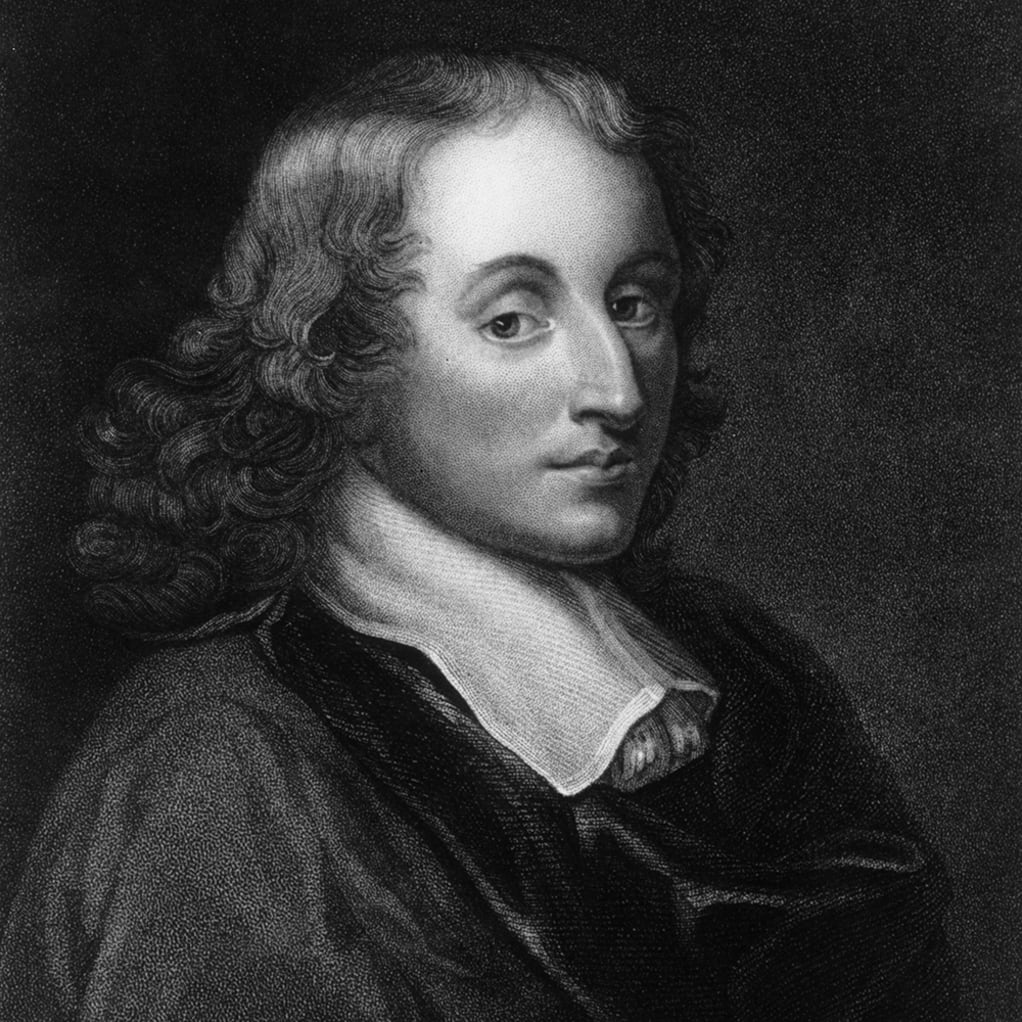
\includegraphics[width=\linewidth]{Images/ApendiceA/PASCAL.jpeg}
\TituloBox{Blaise Pascal:} Nacido el 19 de junio de 1623 en Clermont-Ferrand, Francia; fue un genio precoz y de clara inteligencia, pues su entusiasmo juvenil por la ciencia se materializó en importantes y precursoras aportaciones a la física y a las matemáticas. Siendo aún niño, con solo 12 años, demostró que la suma de los ángulos de un triángulo es siempre igual a 180°. Pese a su frágil salud y corta vida, murió a los 39 años, pero su huella quedó grabada en la historia de la física y de la informática.
}
Uno de los métodos más usados para realizar demostraciones es el Método de Inducción Matemática. Este fue creado por Blaise Pascal en el siglo XVII, aunque el primer matemático que ofreció una demostración formal mediante el uso explicito de la inducción matemática fue el italiano Franciscus Maurolicus (1494-1575). Maurolicus utilizo la inducción para demostrar que para todo entero positivo $n$
$$1 + 3 + 5 + \cdots + (2n-1) = n^2.$$
Dicho método ha servido para demostrar teoremas en distintas áreas de la matemática; como: geometría, teoría de grafos, teoría de números, análisis combinatorio. Una manera informal (pero eficaz) de ver y explicar el Principio de Inducción Matemática es mediante fichas de dominó (véase la figura \ref{fig:INDUCCION}). Imaginemos que tenemos fichas de dominó puestas en una hilera infinita. Si empujamos la primer ficha, esta empujará la segunda ficha; la segunda ficha empujará la tercer ficha; la tercer ficha empujara la cuarta ficha; y así sucesivamente hasta que caigan todas las fichas. En este caso, cada ficha representa un número natural.

Como preliminar, debemos saber que cualquier proposición se puede clasificar como general o particular. Algunos ejemplos de proposiciones generales son:
\begin{enumerate}
    \item Todos los ciudadanos de México tienen derecho a la educación.
    \item Todos los números que terminan en cero son divisibles entre 5.
\end{enumerate}

\newpage
\sideFigure[\label{fig:INDUCCION}Representación del Principio de Inducción]{
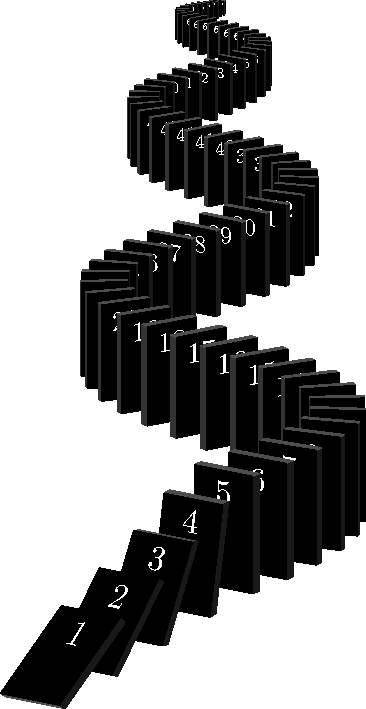
\includegraphics[width=\linewidth]{Images/ApendiceA/uuu.pdf}
}

\noindent Algunos ejemplos de proposiciones particulares son:
\begin{enumerate}
    \item Guinevere tiene derecho a la educación 
    \item 300 es divisible entre 5.
\end{enumerate}
El proceso de obtener una proposición particular de una general se llama \textbf{deducción}. Por ejemplo, si tenemos
\begin{enumerate}
    \item Todos los ciudadanos de México tienen derecho a la educación.
    \item Guinevere es mexicana.
    \item Guinevere tiene derecho a la educación.
\end{enumerate}
entonces de la proposición general (1), junto con la proposición particular (2), se obtiene la proposición particular (3).

El proceso de obtener proposiciones generales de proposiciones particulares se llama \textbf{inducción}. El razonamiento inductivo puede conducir a conclusiones falsas así como a verdaderas. Por ejemplo, si tenemos
\begin{enumerate}
    \item 300 es divisible entre 5.
    \item Todos los números que terminan en cero son divisibles entre 5.
\end{enumerate}
entonces la proposición general (2), obtenida de la proposición particular (1), es verdadera. Pero, si consideramos
\begin{enumerate}
    \item 300 es divisible entre 5.
    \item Todos los números con tres cifras son divisibles entre 5.
\end{enumerate}
entonces la proposición general (2), deducida de la proposición particular (1), es falsa.

En resumen, \emph{La inducción} (o sea, la sugerencia de una idea o una hipótesis) sin duda desempeña en las Matemáticas un papel importante, pero puramente heurístico: permite adivinar cuál debe ser, según todas las apariencias, la solución. Pero las proposiciones matemáticas se demuestran siempre deductivamente. Ningún resultado matemático puede considerarse justo, válido, si no ha sido deducido de las proposiciones de partida.

\noindent\textbf{\fontencoding{T1}\fontfamily{phv}\selectfont\color{black}Problema:\hspace{5pt plus 1pt minus 1pt}} Calcular la suma de los primeros $n$ números impares.

\solucion Los problemas de este tipo se pueden resolver usando una fórmula probada, pero nos interesa resolver el problema sin recurrir a tal fórmula y aplicando el método de la inducción matemática. Para hacerlo, es necesario establecer primero una hipótesis, es decir, tratar de adivinar la solución basándonos en patrones observados. Esto se puede lograr al analizar las sumas parciales de los primeros números impares. Observemos los cálculos de las primeras sumas parciales:
\begin{align*}
    1 & = 1 \\
    1 + 3 & = 4 \\
    1 + 3 + 5 & = 9 \\
    1 + 3 + 5 + 7 & = 16 \\
    1 + 3 + 5 + 7 + 9 & = 25 \\
    1 + 3 + 5 + 7 + 9 + 11 & = 36 \\
    1 + 3 + 5 + 7 + 9 + 11 + 13 & = 49 \\
    1 + 3 + 5 + 7 + 9 + 11 + 13 + 15 & = 64 \\
    1 + 3 + 5 + 7 + 9 + 11 + 13 + 15 + 17 & = 81
\end{align*}\newpage
\marginElement{%
Para $n = 1$:
\begin{center}
    
\begin{tikzpicture}
        \filldraw (0,0) circle (0.2cm);
    \end{tikzpicture}
\end{center}
Para $n = 2$:
\begin{center}
    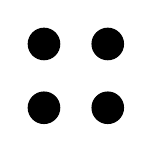
\begin{tikzpicture}
        \def\n{2}
        \def\s{0.81cm}
        \foreach \x in {1,...,\n} {
            \foreach \y in {1,...,\n} {
                \filldraw ({\s*(0.5+(\x-1))},{\s*(\n+0.5-\y)}) circle (0.2cm);
            }
        };
    \end{tikzpicture}
\end{center}
Para $n = 3$:
\begin{center}
    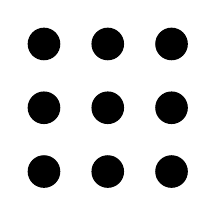
\begin{tikzpicture}
        \def\n{3}
        \def\s{0.81cm}
        \foreach \x in {1,...,\n} {
            \foreach \y in {1,...,\n} {
                \filldraw ({\s*(0.5+(\x-1))},{\s*(\n+0.5-\y)}) circle (0.2cm);
            }
        };
    \end{tikzpicture}
\end{center}
Para $n = 4$:
\begin{center}
    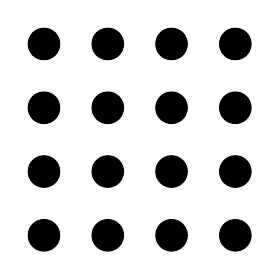
\begin{tikzpicture}
        \def\n{4}
        \def\s{0.81cm}
        \foreach \x in {1,...,\n} {
            \foreach \y in {1,...,\n} {
                \filldraw ({\s*(0.5+(\x-1))},{\s*(\n+0.5-\y)}) circle (0.2cm);
            }
        };
    \end{tikzpicture}
\end{center}
Para $n = 5$:
\begin{center}
    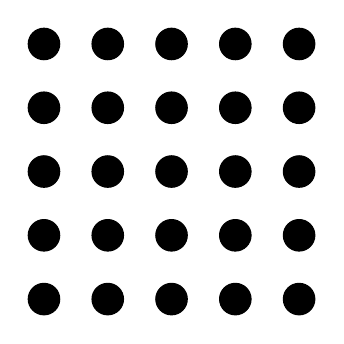
\begin{tikzpicture}
        \def\n{5}
        \def\s{0.81cm}
        \foreach \x in {1,...,\n} {
            \foreach \y in {1,...,\n} {
                \filldraw ({\s*(0.5+(\x-1))},{\s*(\n+0.5-\y)}) circle (0.2cm);
            }
        };
    \end{tikzpicture}
\end{center}
\captionsetup*[figure]{font={normalsize},hypcap=false}%
\captionof{figure}{Representación del modelo
$$1 + 3 + 5 + \cdots + (2n - 1) = n^2$$
cuando $n = 1$, $2$, $3$, $4$, $5$}\label{fig:JEJDJJJJJJDJJ}
}
Cada suma puede representarse en la forma
$$\alpha + \beta + \gamma + \cdots + u = S,$$
donde $u$ representa el último sumando y $S$ la suma. Tanto $u$ como $S$ dependen del número de sumandos, al cual denominaremos con $n$. Estas dependencias se pueden estudiar para identificar patrones o relaciones matemáticas entre las variables involucradas. Dadas estas convenciones, podemos construir dos tablas. La primera tabla nos permitirá explorar la relación entre $n$, el número de sumandos, y $u$, el último término de la suma. La segunda tabla nos ayudará a identificar una posible relación entre $n$ y $S$, la suma total. Estas tablas nos servirán para formular hipótesis iniciales sobre las dependencias funcionales.
\begin{center}
    \begin{minipage}{.4\textwidth}
        \centering
        \begin{tabular}{cc}
            \toprule
            $n$ & $u$ \\
            \midrule
            $1$ & $1$ \\
            $2$ & $3$ \\
            $3$ & $5$ \\
            $4$ & $7$ \\
            $5$ & $9$ \\
            $6$ & $11$ \\
            $7$ & $13$ \\
            $8$ & $15$ \\
            $9$ & $17$ \\
            $10$ & $19$ \\
            \bottomrule
        \end{tabular}
    \end{minipage}
    \begin{minipage}{.4\textwidth}
        \centering
        \begin{tabular}{cc}
            \toprule
            $n$ & $S$ \\
            \midrule
            $1$ & $1$ \\
            $2$ & $4$ \\
            $3$ & $9$ \\
            $4$ & $16$ \\
            $5$ & $25$ \\
            $6$ & $36$ \\
            $7$ & $49$ \\
            $8$ & $64$ \\
            $9$ & $81$ \\
            $10$ & $100$ \\
            \bottomrule
        \end{tabular}
    \end{minipage}
\end{center}
Por lo que se propone el siguiente modelo:
$$1 + 3 + 5 + 7 + 9 + 11 + \cdots + (2n - 1) = n^2.$$
Probemosla por medio de inducción sobre $n$. Llamemos a la suma, $S_n$. Es decir,
$$S_n=1+3+5+7+9+11+\cdots +(2n-1).$$
\begin{enumerate}[label=\roman*.]
    \item Para $n = 1$ es evidente que se cumple, ya que la suma consiste en un solo término, el $1$. El valor de la expresión $n^2$ también es $1$.
    \item Supóngase que la hipótesis se cumple para $n = k$, es decir, $S_k = k^2$.
    \item A partir de (ii), probemos que se cumple para $n = k + 1$, es decir,
    $$S_{k+1} = (k+1)^2.$$
    En efecto, se tiene
    $$S_{k+1} = S_k+(2k+1)$$
    pero $S_k = k^2$, se sigue que
    $$S_{k+1} = k^2+(2k+1)=(k+1)^2.$$
\end{enumerate}
En conclusión, se cumple que $S_n = n^2$. Incluso, para este caso, podemos ver la \emph{demostración visual} de\infoBulle{Una demostración visual implica que la solución de un problema sea accesible de manera clara a través de un diagrama o dibujo, con un mínimo de desarrollo matemático necesario.}
$$1 + 3 + 5 + 7 + 9 + 11 + \cdots + (2n - 1) = n^2$$
como se muestra en la figura \ref{fig:JEJDJJJJJJDJJ}. Aunque no se debe olvidar que esto es una manera visual de ver el comportamiento de una proposición particular. No siempre se puede recurrir a una demostración visual, ya que nos puede llevar a conclusiones falsas. Esto se debe a que las demostraciones visuales suelen depender de la interpretación que hagamos de las imágenes, diagramas o esquemas, lo cual puede resultar engañoso en ciertos contextos. Por ello, la matemática se apoya siempre en la demostración formal y deductiva para garantizar la validez de cualquier proposición. En el caso del ejemplo anterior, aunque la representación visual sea una herramienta poderosa para comprender la regularidad de la suma de los números impares consecutivos, es fundamental corroborar dicho resultado utilizando el Método de Inducción Matemática.

\newpage

\section{Inducción errónea en las matemáticas}

\begin{examplebox}{}{}
    Consideremos el polinomio $f(x)=x^2+x+41$. Si este polinomio se remplaza $x$ por el número $0$, se obtiene el número primo $41$. Si se remplaza $x$ por el número $1$, nuevamente se obtiene un número primo, $43$. Si se sigue este procedimiento para $1$, $2$, $3$, $4$, $5$, $6$; obtenemos que
    \begin{align*}
        f(0) &=41 \\
        f(1) &=43 \\
        f(2) &=47 \\
        f(3) &=53 \\
        f(4) &=61 \\
        f(5) &=71 \\
        f(6) &=83
    \end{align*}
    Basándonos en estos resultados, podría parecer que para todo entero no negativo $x$, el polinomio produce números primos. Sin embargo, esto no es cierto, ya que aunque $x^2 + x + 41$ genera números primos para $f(1)$, $f(2)$, $f(3)$, $\dots$, $f(38)$, $f(39)$, al evaluar $f(40)$ se obtiene $1681$, que es un número compuesto.
\end{examplebox}

\begin{examplebox}{}{}
    El binomio $x^n - 1$, $n \in \NN$, fue estudiado por numerosos matemáticos y factorizado con coeficientes enteros. Al analizar estas factorizaciones para diversos valores de $n$, los matemáticos observaron que los valores absolutos de los coeficientes de los factores nunca superaron el número $1$. Es decir,
    \begin{align*}
        x-1 &=x-1 \\
        x^2-1 &=(x-1)(x+1) \\
        x^3-1 &=(x-1)\left( x^2+x+1 \right) \\
        x^4-1 &=(x-1)(x+1)\left(x^2+1\right) \\
        &\vdots 
    \end{align*}
    Se construyeron tablas de coeficientes, y en cada caso los coeficientes cumplían la propiedad mencionada. Sin embargo, no se logró probar la validez de la proposición para todos los valores de $n$ hasta que V. Ivanov resolvió el problema en 1941. Si $n < 105$, el binomio $x^n - 1$ cumple la propiedad, pero uno de los factores de $x^{105} - 1$ es el polinomio.
    \begin{align*}
        x^{48} & +x^{47}+x^{46}-x^{43}-x^{42}-2x^{41}-x^{40}-x^{39}+x^{36}+x^{35}+x^{34}+x^{33} \\
        &+x^{32}+x^{31}-x^{28}-x^{26}-x^{24}-x^{22}-x^{20}+x^{17}+x^{16}+x^{15}+x^{14} \\
        &+x^{13}+x^{12}-x^9-x^8-2x^7-x^6-x^5+x^2+x+1
    \end{align*}
    que ya no tiene esta propiedad.
\end{examplebox}

\begin{examplebox}{}{}
    Gottfried W. Leibniz, destacado matemático alemán del siglo XVII, demostró que, para cualquier entero positivo $n$, el número $n^3 - n$ es divisible por $3$, $n^5 - n$ es divisible por $5$ y $n^7 - n$ es divisible por $7$. Concluyó que para todo $k$ impar y cualquier $n$ natural, $n^k - n$ sería divisible por $k$. Sin embargo, pronto descubrió que $2^9 - 2 = 510$ no es divisible por $9$.
\end{examplebox}

\begin{examplebox}{}{}
    Un error del mismo carácter cometió D. Aleksandrovich Grave, conocido matemático soviético, al suponer que para todo primo $p$ el número $2^{p-1} - 1$ no es divisible por $p^2$. El cálculo directo confirmaba esta hipótesis para todos los números $p$ menores que mil. Sin embargo, pronto se comprobó que $2^{1092} - 1$ es divisible por $1093^2$ (1093 es un número primo); o sea, la hipótesis de Grave resultó errónea.
\end{examplebox}

\newpage

\begin{examplebox}{}{}
    Consideremos los números del tipo
    $$2^{2^n} + 1.$$
    Para $n = 0, 1, 2, 3, 4$, los números $3$, $5$, $17$, $257$, $65 \, 537$ son primos. Pierre de Fermat, matemático francés del siglo XVII, afirmó que todos estos números eran primos. Sin embargo, L. Euler descubrió en el siglo XVIII que
    $$2^{2^5} + 1 = 4 \, 294 \, 967 \, 297 = (641)(6 \, 700 \, 417)$$
    es un número compuesto.
\end{examplebox}

\section{El principio de la inducción matemática}

\begin{tcolorbox}[
    % Estilo del teorema
    theorem style=change apart,
    enhanced,
    lower separated=false,
    breakable,
    % Bordes
    boxrule=0pt,
    frame hidden,
    % Colores
    colback=black!7!white,
    coltitle=black,
    % Título
    boxed title style={colframe=white, colback=white, boxrule=0pt},
    % Texto
    fontupper=\normalsize,
    before upper={\abovedisplayskip=8pt\belowdisplayskip=8pt},
    % Márgenes
    left=1mm,
    right=1mm,
    top=1mm,
    bottom=1mm,
    % Esquinas
    sharp corners,
    % Superposición
    overlay={
        \node[left, font=\bfseries\color{black}\fontencoding{T1}\fontfamily{phv}\selectfont,minimum width=2cm, anchor=east, xshift=-0.5\marginparsep, yshift=-0.348cm] at (frame.north west) {Principio de Inducción:};
    }
]
    Sea $P$ una propiedad cualquiera. Tenemos que $P(1), P(2), P(3), P(4), \dots$ es un conjunto de propiedades para cada número natural tal que:
    \begin{enumerate}[label=\roman*., topsep=6pt, itemsep=0pt]
        \item $P(1)$ es cierta.
        \item Si $P(n)$ es cierta, entonces $P(n+1)$ es cierta.
    \end{enumerate}
    Entonces $P(n)$ es cierta para toda $n \in \NN$.
\end{tcolorbox}

\begin{examplebox}{}{}
    Demostrar que
    $$1+2+\cdots +n=\frac{n(n+1)}{2}, \forall n \in \NN.$$
    \demostracion Claramente $n=1$, satisface la fórmula, ya que
    \begin{align*}
        1 &=\frac{1(1+1)}{2} \\
        1 &=1
    \end{align*}
    lo cual es verdadero. Supongamos que la fórmula se cumple para $n=k$, es decir, supongamos que
    $$1+2+\cdots +k=\frac{k(k+1)}{2}.$$
    Demostraremos a partir de lo dicho anteriormente que la fórmula se cumple para $n=k+1$. Es decir, probaremos que
    $$1+2+\cdots +k=\frac{(k+1)(k+2)}{2}.$$
    En efecto, por hipótesis de inducción
    $$1+2+\cdots +k=\frac{k(k+1)}{2}.$$
    Entonces
    \begin{align*}
        1+2+\cdots +k+k+1 &=\frac{k(k+1)}{2}+k+1 \\
        &=\frac{k(k+1)+2(k+1)}{2} \\
        &=\frac{(k+1)(k+2)}{2}
    \end{align*}
    es decir
    $$1+2+\cdots +k+1=\frac{(k+1)(k+2)}{2}.$$
    Por tanto,
    $$1+2+\cdots +n=\frac{n(n+1)}{2}, \forall n \in \NN.$$
\end{examplebox}

\newpage

\begin{examplebox}{}{}
    Demostrar que
    $$1^3+2^3+\cdots +n^3=(1+2 +\cdots +n)^2, \forall n \in \NN.$$
    \demostracion Claramente $n=1$ satisface la fórmula, ya que al sustituir $n$ por $1$ se tiene
    \begin{align*}
        1^3 &=(1)^2 \\
        1 &=1
    \end{align*}
    lo cual es verdadero. Notemos por el ejercicio anterior que
    $$1+2+\cdots +n=\frac{n(n+1)}{2}$$
    entonces tenemos que
    $$1^3+2^3+\cdots +n^3=\left( \frac{n(n+1)}{2} \right)^2.$$
    Así pues, supongamos que la fórmula cumple para $n=k$, es decir
    $$1^3+2^3+\cdots +k^3=\left( \frac{k(k+1)}{2} \right)^2.$$
    Demostraremos a partir de lo dicho anteriormente que la fórmula se cumple para $n=k+1$. Es decir, probaremos que
    $$1^3+2^3+\cdots +k^3=\left( \frac{k(k+1)}{2} \right)^2.$$
    En efecto: por hipótesis de inducción
    \begin{align*}
        1^3 +2^3+ \cdots +k^3+(k+1)^3 &=\left( \frac{k(k+1)}{2} \right)^2 +(k+1)^3\\
        &=\frac{k^2(k+1)^2}{4}+(k+1)^3 \\
        &=\frac{k^2(k+1)^2+4(k+1)^3}{4} \\
        &=\frac{(k+1)^2\big(k^2+4(k+1)\big)}{4} \\
        &=\frac{(k+1)^2 (k^2+4k+4)}{4} \\
        &=\frac{(k+1)^2(k+2)^2}{4} \\
        &=\left(\frac{(k+1)(k+2)}{2}\right)^2
    \end{align*}
    Por tanto,
    $$1^3+2^3+\cdots +n^3=(1+2+\cdots +n)^2, \forall n \in \NN.$$
\end{examplebox}

El método de la inducción matemática no es el único procedimiento para demostrar que una propiedad $P$ se cumple para cada número natural. Existen otros métodos que también permiten establecer la validez de propiedades matemáticas, aunque la inducción es particularmente útil por su estructura sistemática y lógica. No obstante, el hecho de no poder demostrar que $P$ se cumple para todos los números naturales no implica que $P$ sea falsa, sino únicamente que, hasta el momento, no se ha encontrado una demostración válida. Demostrar que una propiedad $P$ es falsa requiere una estrategia diferente, y basta con encontrar un \emph{contraejemplo}, es decir, un caso específico donde $P$ no se cumpla. Este procedimiento es directo y concluyente, pues un solo contraejemplo es suficiente para refutar la validez universal de una propiedad. \infoBulle{Varios ejemplos de dar un contraejemplo, fueron mostrados en la sección anterior, donde se observo cómo un contraejemplo puede invalidar una afirmación aparentemente general.}

\newpage

\begin{examplebox}{}{}
    Demostrar que
    $$1^2+2^2+\cdots +n^2=\frac{n(n+1)(2n+1)}{6}, \forall n \in \NN.$$
    \demostracion Claramente $n=1$ satisface la fórmula, ya que
    \begin{align*}
        1^2 &=\frac{1(1+1)(2\cdot 1+1)}{6} \\
        1 &=1
    \end{align*}
    Supongamos que la fórmula se cumple para $n=k$, es decir, supongamos que
    $$1^2+2^2+\cdots +k^2=\frac{k(k+1)(2k+1)}{6}$$
    Demostraremos a partir de lo dicho anteriormente que la fórmula se cumple para $n=k+1$. Es decir, probaremos que
    $$1^2+2^2+\cdots +(k+1)^2=\frac{(k+1)(k+2)(2k+3)}{6}.$$
    En efecto: por hipótesis de inducción
    $$1^2+2^2+\cdots +k^2=\frac{k(k+1)(2k+1)}{6}.$$
    Entonces
    \begin{align*}
        1^2 +2^2+\cdots +k^2+(k+1)^2 &=\frac{k(k+1)(2k+1)}{6}+(k+1)^2 \\
        &=\frac{k(k+1)(2k+1)+6(k+1)^2}{6} \\
        &=\frac{(k+1)\big(k(2k+1)+6(k+1)\big)}{6} \\
        &=\frac{(k+1)(2k^2+7k+6)}{6} \\
        &=\frac{(k+1)(k+2)(2k+3)}{6}
    \end{align*}
    Por tanto,
    $$1^2+2^2+\cdots +n^2=\frac{n(n+1)(2n+1)}{6}, \forall n \in \NN.$$
\end{examplebox}

En resumen, para demostrar que una propiedad $P$ se cumple para cada número natural, se emplea un procedimiento llamado \emph{demostración por inducción matemática}. Es decir, si $\NN$ es el conjunto de los números naturales y $A \subset \NN$ tal que:
\begin{enumerate}[label=\roman*.]
    \item $1 \in A$.
    \item $k \in A \Longrightarrow k+1 \in A$. Entonces $A = \NN$.
\end{enumerate}

Sin embargo, en ciertas demostraciones por inducción, resulta útil emplear el siguiente principio:

\begin{tcolorbox}[
    % Estilo del teorema
    theorem style=change apart,
    enhanced,
    lower separated=false,
    breakable,
    % Bordes
    boxrule=0pt,
    frame hidden,
    % Colores
    colback=black!7!white,
    coltitle=black,
    % Título
    boxed title style={colframe=white, colback=white, boxrule=0pt},
    % Texto
    fontupper=\normalsize,
    before upper={\abovedisplayskip=8pt\belowdisplayskip=8pt},
    % Márgenes
    left=1mm,
    right=1mm,
    top=1mm,
    bottom=1mm,
    % Esquinas
    sharp corners,
    % Superposición
    overlay={
        \node[left, font=\bfseries\color{black}\fontencoding{T1}\fontfamily{phv}\selectfont,minimum width=2cm, anchor=east, xshift=-0.5\marginparsep, yshift=-0.348cm] at (frame.north west) {Inducción Modificado:};
    }
]
    Si $A$ es un subconjunto de los números naturales tal que
    \begin{enumerate}[label=\roman*., topsep=6pt, itemsep=0pt]
        \item $1 \in A$.
    \item Si $1, 2, \dots , n \in A$, implica que $n+1 \in A$.
    \end{enumerate}
    Entonces $A = \NN$.
\end{tcolorbox}

Sea $P(n)$ una propiedad cualquiera. Si se quiere demostrar que $P(n)$ es cierta para toda $n \in \NN$, es decir, $A:=\left\lbrace n \in \NN \mid P(n) \text{ es cierta} \right\rbrace = \NN$
es suficiente mostrar que $A$ satisface las dos hipótesis del Principio de Inducción Modificado.

\newpage

Podría suceder que $P(n)$ no sea verdadera para todos los números naturales, pero existe cierto número natural $i$ tal que $P(k)$ es verdadera para toda $i \leq k$. Se puede utilizar también el Principio de Inducción Modificado considerando al conjunto
$$A:=\left\lbrace n \in \NN \mid P(n+i) \text{ es cierta} \right\rbrace $$
en cuyo caso se reduce a demostrar que:
\begin{enumerate}[label=\roman*.]
    \item $P(i)$ es verdadera.
    \item Si $P(k)$ es cierta para $k=i, i+1, \dots, i+n$, entonces $P\big( i+(n+1) \big)$ es cierta.
\end{enumerate}

\begin{prop}{}{}
    El Principio de Inducción y el Principio de Inducción Modificado son equivalentes.

    \tcblower
    \demostracion Se deja como ejercicio al lector.
\end{prop}

\section{El principio de buen orden}

\begin{tcolorbox}[
    % Estilo del teorema
    theorem style=change apart,
    enhanced,
    lower separated=false,
    breakable,
    % Bordes
    boxrule=0pt,
    frame hidden,
    % Colores
    colback=black!7!white,
    coltitle=black,
    % Título
    boxed title style={colframe=white, colback=white, boxrule=0pt},
    % Texto
    fontupper=\normalsize,
    before upper={\abovedisplayskip=8pt\belowdisplayskip=8pt},
    % Márgenes
    left=1mm,
    right=1mm,
    top=1mm,
    bottom=1mm,
    % Esquinas
    sharp corners,
    % Superposición
    overlay={
        \node[left, font=\bfseries\color{black}\fontencoding{T1}\fontfamily{phv}\selectfont,minimum width=2cm, anchor=east, xshift=-0.5\marginparsep, yshift=-0.348cm] at (frame.north west) {Principio de Buen Orden:};
    }
]
    Si $A$ es un subconjunto no vacío de los números naturales, entonces existe $a \in A$ tal que $a \leq x$, $\forall x \in A$, es decir, $A$ tiene elemento mínimo, que es $a$. Al elemento mínimo de $A$, también llamado primer elemento de $A$, se le denota por $\min A$, es decir, $a = \min A$.
\end{tcolorbox}

\begin{examplebox}{}{}
    Consideremos el conjunto $A = \{5, 10, 15, 20, 25, 30\}$, un subconjunto no vacío de los números naturales. Por el Principio de Buen Orden, este conjunto tiene un elemento mínimo, que en este caso es $5$, ya que es el menor de todos sus elementos. Por lo tanto,
    $$a = \min A = 5.$$
\end{examplebox}

\begin{examplebox}{}{}
    Todo número natural puede ser representado como una suma de unos.

    \tcblower
    \demostracion Queremos demostrar que para cualquier número natural $n$,
    $$n = \underbrace{1 + 1 + \cdots + 1}_{n \text{ veces}}$$
    Consideremos el conjunto $A$ de todos los números naturales que no pueden ser escritos como una suma de unos. Es decir:
    $$A = \{ n \in \NN \mid n \text{ no puede ser escrito como una suma de unos} \}$$
    Según el Principio de Buen Orden, si $A$ no es vacío, entonces debe tener un elemento mínimo. Sea $m$ el elemento mínimo de $A$. Por definición, $m$ no puede ser escrito como una suma de unos. Ahora, consideremos $m - 1$. Si $m - 1 = 0$, entonces $m = 1$. Sin embargo, $1$ puede ser escrito como una suma de un único $1$, es decir, $1 = 1$. Esto es una contradicción porque asumimos que $m$ no puede ser escrito como una suma de unos. Si $m - 1$ es un número natural positivo, entonces $m - 1$ debe ser escribible como una suma de unos, ya que $m$ es el mínimo elemento de $A$ y $m - 1 < m$. Supongamos entonces que $m - 1$ puede ser escrito como
    $$m - 1 = 1 + 1 + \cdots + 1 \quad \text{ con } m - 1 \text{ unos}$$
    Al agregar un $1$ más a esta suma, obtenemos
    $$m = (1 + 1 + \cdots + 1) + 1 \quad \text{ con } m \text{ unos}$$
    Esto demuestra que $m$ puede ser escrito como una suma de unos, lo cual es una contradicción porque $m$ se suponía que no podía ser escrito como una suma de unos. Dado que suponer que $A$ no es vacío nos lleva a una contradicción, debemos concluir que $A$ es vacío. Esto significa que no existe ningún número natural que no pueda ser escrito como una suma de unos. Por lo tanto, hemos demostrado que cualquier número natural $n$ puede ser representado como una suma de unos.
\end{examplebox}

\newpage

\begin{examplebox}{}{}
    Todo número natural mayor que uno puede ser descompuesto en un producto de números primos.

    \tcblower
    \demostracion Supongamos que existe un conjunto $B$ de números naturales mayores que $1$ que no pueden ser descompuestos de esta forma. Si $B \neq \emptyset$, sea $n$ el elemento mínimo de $B$. Si $n$ es primo, ya es un producto de un solo número primo, contradiciendo que $n \in B$. Por lo tanto, $n$ debe ser compuesto, es decir, $n = a \cdot b$ con $1 < a, b < n$. Como $a, b < n$ y $n$ es el mínimo de $B$, $a$ y $b$ no están en $B$ y pueden ser descompuestos en productos de números primos. Así,
    $$n = a \cdot b = (p_1 \cdot p_2 \cdots p_k) \cdot (q_1 \cdot q_2 \cdots q_m)$$
    donde $a = p_1 \cdot p_2 \cdots p_k$ y $b = q_1 \cdot q_2 \cdots q_m$ son productos de números primos. Esto contradice la suposición de que $n$ no puede ser descompuesto en un producto de números primos, por lo que $B = \emptyset$. Es decir, no existe ningún número natural mayor que $1$ que no pueda ser descompuesto en un producto de números primos. Por lo tanto, hemos demostrado que todo número natural $n > 1$ puede ser descompuesto en un producto de números primos, utilizando el Principio del Buen Orden.
\end{examplebox}

\begin{theorem}{}{}
    El Principio de Buen Orden es equivalente al Principio de Inducción

    \tcblower
    \demostracion
    \begin{enumerate}[topsep=4pt, itemsep=0pt]
        \item[$\Rightarrow$)] El Principio de Buen Orden implica el Principio de Inducción: Supongamos que existe $M \subset \NN$ tal que
        \begin{enumerate}[label=\roman*)]
            \item $1 \in M$,
            \item $k \in M \Longrightarrow k + 1 \in M$.
        \end{enumerate}
        Supongamos que $M \neq \NN$. Sea $M^C = \NN - M$ el complemento de $M$. Como $M \neq \NN$, entonces $M^C \neq \emptyset$, por lo tanto existe $a \in M^C$ tal que $a \leq x$, $\forall x \in M^C$. Como $1 \in M$, entonces $1 \notin M^C$, así que $a \neq 1$, por tanto existe $k \in \NN$ tal que $k + 1 = a$, entonces $k \notin M^C$ y por tanto $k \in M$, de donde se sigue, aplicando (ii), que $k + 1 = a \in M$, lo cual es una contradicción, pues $a \in M^C$ y $M \cap M^C = \emptyset$. Por tanto, si $M \subset \NN$ y se cumplen (i) y (ii), se debe cumplir que $M = \NN$.
        \item[$\Leftarrow$)] El Principio de Inducción implica el Principio de Buen Orden: Consideremos $A \subset \NN$ con $A \neq \emptyset$. Supongamos que $A$ no tiene elemento mínimo, es decir, supongamos que $\forall k \in A$, existe $x \in A$ tal que $x < k$. Consideremos a $B = \{ y \in \NN \mid y < x$, $\forall x \in A \}$. Ya que $x \nless x$, $\forall x \in A$, entonces tenemos que $B \cap A = \emptyset$. Demostremos ahora, aplicando el Principio de Inducción Matemática, que $B = \NN$. Por como se define, es claro que $B \subset \NN$.
        \begin{enumerate}[label=\roman*)]
            \item Afirmamos que $1 \in B$. Esto ya que $1 \leq n$, $\forall n \in \NN$, entonces $1 \leq x$, $\forall x \in A$. Además $1 \notin A$, ya que si $1 \in A$, entonces $1 = \min A$, lo que contradice la suposición de que $A$ no tiene elemento mínimo. Por tanto, $1 < x$, $\forall x \in A$, y en consecuencia $1 \in B$.
            \item Supongamos que $n \in B$, es decir, supongamos que $n < x$, $\forall x \in A$.
            \item Probaremos a partir de (ii) que $n + 1 \in B$. Si $n \in B$ entonces $n < x$, $\forall x \in A$, por tanto $n + 1 \leq x$, $\forall x \in A$, y por tanto $n + 1 \in B$.
        \end{enumerate}
        Por (i), (ii), (iii), $B = \NN$, y como $A \subset \NN = B$ y $B \cap A = \emptyset$, entonces $A = \emptyset$, lo cual contradice que $A \neq \emptyset$. En consecuencia, si $A \subset \NN$ y $A \neq \emptyset$, entonces $A$ debe tener elemento mínimo.
    \end{enumerate}
\end{theorem}

Al utilizar el Principio de Buen Orden, se pueden abordar problemas complejos al enfocarse en el elemento más pequeño de un conjunto, lo cual a menudo conduce a contradicciones que invalidan suposiciones erróneas. Este enfoque simplifica el análisis lógico al reducir un problema abstracto a un caso específico y manejable, facilitando la identificación de inconsistencias en las suposiciones iniciales.

\newpage

\section{Más ejemplos de inducción}
\vspace{-0.15cm}
\begin{examplebox}{}{}
    Demostremos que para toda $n \in \NN$,
    $$\int_{0}^{\infty} e^{-x}x^{n} dx=n!$$
    Pero antes, recordemos la siguiente propiedad:
    $$\lim_{x \to \infty} e^{px}=0, \text{ si } p<0.$$
    Así pues, si $n = 0$, entonces
    \begin{align*}
        \int_{0}^{\infty} e^{-x} dx & = \left. -e^{-x} \right|_{0}^{\infty} \\
        & = - \lim_{x \rightarrow \infty} e^{-x} + e^{-0} \\
        & = 0!
    \end{align*}
    Si $n = 1$, se procede por integración por partes. Tomando
    $$u = x \quad \text{ y } \quad dv = e^{-x} dx$$
    obtenemos
    $$du = dx \quad \text{ y } \quad v = -e^{-x}.$$
    Entonces
    \begin{align*}
        \int_0^{\infty} e^{-x}x & = \left. -xe^{-x} \right|_{0}^{\infty} + \int_0^{\infty} e^{-x} dx \\
        & = - \lim_{x \to \infty} xe^{-x} + (0)e^{-0} + 1 \\
        & = 1!
    \end{align*}
    Supongamos que se cumple para $n=k$, es decir,
    $$\int_{0}^{\infty} e^{-x}x^{k} dx = k!.$$
    Demostraremos a partir lo dicho anteriormente, que la propiedad se cumple para $n=k+1$, es decir,
    $$\int_{0}^{\infty} e^{-x}x^{k+1} dx = (k + 1)!.$$
    Procederemos por integración por partes. Así pues, tomando a
    $$u = x^{k+1} \quad \text{ y } \quad dv = e^{-x} dx$$
    obtenemos
    $$du = (k+1)x^k dx \quad \text{ y } \quad v = -e^{-x}.$$
    Entonces
    \begin{align*}
        \int_{0}^{\infty} e^{-x}x^{k+1} dx &= \left. -x^{k+1}e^{-x} \right|_{0}^{\infty} + (k+1) \int_{0}^{\infty} e^{-x} x^k dx \\
        & = - \lim_{x \rightarrow \infty} x^{k+1}e^{-x}+(0)^{k+1}e^{-0}+(k+1)k! \\
        & = - \lim_{x \rightarrow \infty} \frac{(k+1)!}{e^x} +(k+1)k! \\
        & = (k + 1)!
    \end{align*}
    Por tanto,
    $$\int_{0}^{\infty} e^{-x}x^{n} dx = n!, \forall n \in \NN.$$
\end{examplebox}

\newpage

\begin{examplebox}{}{mediageometricaaritmetica}
    Si $a_1, a_2, \dots, a_n$ son números reales positivos, demuestre que
    \begin{equation}
        \sqrt[n]{a_1\cdot a_2 \cdots a_n} \leq \frac{a_1+a_2+\cdots +a_n}{n}. \label{A1}
    \end{equation}

    \tcblower
    \demostracion 
    \begin{enumerate}[label=\roman*., topsep=6pt, itemsep=0pt]
        \item Para $n = 2$, la desigualdad \eqref{A1} da
        \begin{equation}
            \sqrt{a_1a_2} \leq \frac{a_1+a_2}{2}. \label{A2}
        \end{equation}
        Es fácil obtener esta desigualdad a partir de esta otra
        $$\left( \sqrt{a_1} - \sqrt{a_2} \right)^2 \geq 0,$$
        válida para cualesquiera $a_1$, $a_2$ números reales positivos. La desigualdad \eqref{A2} tiene una interpretación geométrica: en una recta $AB$, tomemos los segmentos $a_1$ y $a_2$, y construyamos una circunferencia con diámetro $a_1 + a_2$. Aquí, $\dfrac{a_1 + a_2}{2}$ es el radio de la circunferencia, y $\sqrt{a_1a_2}$ es la mitad de la cuerda perpendicular al diámetro en el punto donde se unen $a_1$ y $a_2$ (véase la figura \ref{fig:JNVKJYYS}). Esto demuestra \eqref{A2}.
        \item Supongamos que la desigualdad \eqref{A1} se cumple para $n = k$. Demostremos que, entonces, también se cumple para $n = 2k$. En efecto,
        \begin{align*}
            \sqrt[2k]{a_1\cdot a_2 \cdots a_{2k}} & = \sqrt{\sqrt[k]{a_1 \cdot a_2 \cdots a_k}\sqrt[k]{a_{k+1} \cdots a_{2k}}} \\
            & \leq \frac{\sqrt[k]{a_1 \cdot a_2 \cdots a_k} + \sqrt[k]{a_{k+1} \cdots a_{2k}}}{2} \\
            & \leq \displaystyle\frac{\displaystyle\frac{a_1+a_2+\cdots +a_k}{k} +\displaystyle\frac{a_{k+1}+\cdots+a_{2k}}{k}}{2} \\
            & = \frac{a_1+a_2+\cdots+a_k+\cdots+a_{2k}}{2k}
        \end{align*}
        Como ya demostramos la desigualdad \eqref{A1} para $n = 2$, se cumple también para $n = 4$, $8$, $16$, $\dots$, es decir, para $n = 2^s$ con $s \in \NN$.
        \item Para demostrar que la desigualdad \eqref{A1} se cumple para cualquier número natural $n$, probemos que si se cumple para $n = k$, también se cumple para $n = k-1$. Sean pues, $a_1$, $a_2$, $\dots$, $a_{k-1} \in \RR[+]$. Sea $\lambda \in \RR[+]$, entonces
        $$\sqrt[k]{a_1 \cdot a_2 \cdots a_{k-1}\lambda} \leq \frac{a_1+a_2+\cdots+a_{k-1}+\lambda}{k}.$$
        Determinemos $\lambda$ de modo que
        $$\frac{a_1+a_2+\cdots+a_{k-1}+\lambda}{k} = \frac{a_1+a_2+\cdots+a_{k-1}}{k-1},$$
        o sea, pongamos
        $$\lambda = \frac{a_1+a_2+\cdots+a_{k-1}}{k-1}.$$
        Tenemos
        $$\sqrt[k]{\frac{a_1 \cdot a_2 \cdots a_{k-1} (a_1+a_2+\cdots+a_{k-1})}{k-1}} \leq \frac{a_1+a_2+\cdots+a_{k-1}}{k-1},$$
        es decir,
        $$\sqrt[k-1]{a_1 \cdot a_2 \cdots a_{k-1}} \leq \frac{a_1+a_2+\cdots+a_{k-1}}{k-1}.$$
        Sea ahora $m \in \NN$. Si $m = 2^s$, la desigualdad se cumple por (ii). Si $m \neq 2^s$, elegimos $s$ tal que $m < 2^s$; entonces, por (ii) y (iii), la desigualdad también se cumple para $n = m$.
    \end{enumerate}
    Por tanto, se cumple que
    $$\sqrt[n]{a_1\cdot a_2 \cdots a_n} \leq \frac{a_1+a_2+\cdots +a_n}{n}, \forall a_1, a_2, \dots, a_n \in \RR[+], \forall n \in \NN.$$
\end{examplebox}

\infoBulle{La expresión \eqref{A1} se le conoce como \emph{desigualdad entre la media geométrica y la media aritmética}. Obsérvese que si
$$a_1 = a_2 = \cdots = a_n$$
entonces $$\sqrt[n]{a_1\cdot a_2 \cdots a_n} = \frac{a_1+a_2+\cdots +a_n}{n}.$$En caso contrario, $$\sqrt[n]{a_1\cdot a_2 \cdots a_n} < \frac{a_1+a_2+\cdots +a_n}{n}.$$}
\sideFigure[\label{fig:JNVKJYYS}]{
\begin{center}
    \begin{tikzpicture}[baseline=(current bounding box.north)]
        \begin{scope}
            \clip (-2.1,-0.01) rectangle (2.1,2.1);
            \draw[thick] (0,0) circle (2);
            \draw[thick] (-2,0) -- (2,0);
            \draw (1,0) -- (1,1.7) -- (0,0);
            \draw[stealth-stealth] (1.4,0) -- (1.4,1.73);
            \node[fill=white,rotate=90] at (1.4,0.6) {$\sqrt{a_1a_2}$};
        \end{scope}
        \draw[stealth-stealth] (-2,-0.5) -- (1,-0.5);
        \node at (-0.5,-0.5) [below] {$a_1$};
        \draw[stealth-stealth] (1,-0.5) -- (2,-0.5);
        \node at (1.5,-0.5) [below] {$a_2$};
        \draw[stealth-stealth] (-0.3,0.1) -- (0.7,1.83);
        \node[fill=white,rotate=60] at (0.1,1) {$\dfrac{a_1+a_2}{2}$};
    \end{tikzpicture}
\end{center}
}

\newpage

\begin{examplebox}{}{}
    Hallar una expresión para la suma
    $$1 \cdot 1! + 2 \cdot 2! + 3 \cdot 3! + \cdots + n \cdot n!.$$

    \tcblower
    \demostracion Llamemos a la suma anterior, $S_n$. Es decir
    $$S_n=1 \cdot 1! + 2 \cdot 2! + 3 \cdot 3! + \cdots + n \cdot n!.$$
    Para entender mejor esta suma, calculemos las primeras sumas parciales:
    \begin{align*}
        1 \cdot 1! & = 1 \\
        1 \cdot 1! + 2 \cdot 2! & = 5 \\
        1 \cdot 1! + 2 \cdot 2! + 3 \cdot 3! & = 23 \\
        1 \cdot 1! + 2 \cdot 2! + 3 \cdot 3! + 4 \cdot 4! & = 119 \\
        1 \cdot 1! + 2 \cdot 2! + 3 \cdot 3! + 4 \cdot 4! + 5 \cdot 5! & = 719 \\
        1 \cdot 1! + 2 \cdot 2! + 3 \cdot 3! + 4 \cdot 4! + 5 \cdot 5! + 6 \cdot 6! & = 5039 \\
        1 \cdot 1! + 2 \cdot 2! + 3 \cdot 3! + 4 \cdot 4! + 5 \cdot 5! + 6 \cdot 6! + 7 \cdot 7! & = 40 \, 319
    \end{align*}
    Examinando los resultados anteriores, podemos notar un patrón que se resume en
    \begin{align*}
        S_1 & = 2! - 1 \\
        S_2 & = 3! - 1 \\
        S_3 & = 4! - 1 \\
        S_4 & = 5! - 1 \\
        S_5 & = 6! - 1 \\
        S_6 & = 7! - 1 \\
        S_7 & = 8! - 1
    \end{align*}
    Esto conduce a la hipótesis
    $$S_n = (n + 1)! - 1.$$
    Verifiquemos dicha hipótesis.
    \begin{enumerate}[label=\roman*., topsep=6pt, itemsep=0pt]
        \item La hipótesis se cumple para $n=1$, pues
        $$S_1=1 \cdot 1!=2!-1.$$
        \item Supongamos que la hipótesis se cumple para $n=k$, es decir,
        $$S_k=(k+1)!-1.$$
        \item A partir de (ii), probemos que se cumple para $n=k+1$, es decir,
        $$S_{k+1}=(k+2)!-1.$$
        En efecto,
        \begin{align*}
            S_{k+1} &= S_k + (k+1) \cdot (k+1)! \\
            &=[(k+1)!-1]+(k+1) \cdot (k+1)! \\
            &=(k+1)![1+(k+1)]-1 \\
            &=(k+1)!(k+2)-1 \\
            &=(k+2)!-1
        \end{align*}
    \end{enumerate}
    Por tanto, se cumple que
    $$1 \cdot 1! + 2 \cdot 2! + 3 \cdot 3! + \cdots + n \cdot n! = (n+1)!-1, \forall n \in \NN .$$
\end{examplebox}

\newpage

\begin{examplebox}{}{}
    Sea
    $$\makecell{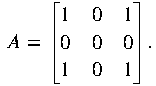
\includegraphics[page=1]{Externalizacion/A1/MatricesA1.pdf}}$$
    Encuentre $A^n$ para toda $n \in \NN$.

    \tcblower
    \solucion Deseamos calcular $A^n$. Para esto, primero calculemos varias potencias de esta matriz como sigue:
    \begin{matrizn}
        \makecell{\includegraphics[page=2]{Externalizacion/A1/MatricesA1.pdf}}
    \end{matrizn}
    Observemos que existe un patrón, así que proponemos
    \begin{matrizn}
        \makecell{\includegraphics[page=3]{Externalizacion/A1/MatricesA1.pdf}}
    \end{matrizn}
    Probemosla por medio de inducción sobre $n$.
    \begin{enumerate}[label=\roman*., topsep=6pt, itemsep=0pt]
        \item Para $n = 1$ es evidente que se cumple.
        \item Supongamos que la hipótesis se cumple para $n = k$, es decir,
        \begin{matrizn}
            \makecell{\includegraphics[page=4]{Externalizacion/A1/MatricesA1.pdf}}
        \end{matrizn}
        \item A partir de (ii), probemos que se cumple para $n = k + 1$, es decir,
        \begin{matrizn}
            \makecell{\includegraphics[page=5]{Externalizacion/A1/MatricesA1.pdf}}
        \end{matrizn}
        En efecto, sabiendo que $A^{k + 1} = A^kA$, se tiene
        \begin{matrizn}
            \makecell{\includegraphics[page=6]{Externalizacion/A1/MatricesA1.pdf}}
        \end{matrizn}
    \end{enumerate}
    Por lo tanto, se cumple que
    \begin{matrizn}
        \makecell{\includegraphics[page=7]{Externalizacion/A1/MatricesA1.pdf}}
    \end{matrizn}
\end{examplebox}

\newpage

Esta fórmula no solo proporciona una expresión general para $A^n$, sino que también destaca cómo el comportamiento de las potencias de matrices puede describirse de manera sistemática y predecible mediante patrones algebraicos. El siguiente ejemplo, ilustra cómo se aplica este enfoque en un caso general.

\begin{examplebox}{}{}
    Sea $a \in \RR$ y sea
    $$A = \begin{bmatrix}
        a & 1 \\
        0 & a
    \end{bmatrix}.$$
    Encuentre $A^n$ para toda $n \in \NN$.

    \tcblower
    \solucion Deseamos calcular $A^n$. Para ello, comenzaremos calculando varias potencias iniciales de la matriz $A$ y observaremos si se sigue un patrón:
    \begin{matrizn}
        \makecell{\includegraphics[page=8]{Externalizacion/A1/MatricesA1.pdf}}
    \end{matrizn}
    A partir de estos cálculos iniciales, observamos que las potencias de $A$ parecen seguir un patrón general. Conjeturamos que
    \begin{matrizn}
        \makecell{\includegraphics[page=9]{Externalizacion/A1/MatricesA1.pdf}}
    \end{matrizn}
    Probemosla por medio de inducción sobre $n$.
    \begin{enumerate}[label=\roman*., topsep=6pt, itemsep=0pt]
        \item Para $n = 1$ es evidente que se cumple.
        \item Supongamos que la hipótesis se cumple para $n = k$, es decir,
        \begin{matrizn}
            \makecell{\includegraphics[page=10]{Externalizacion/A1/MatricesA1.pdf}}
        \end{matrizn}
        \item A partir de (ii), probemos que se cumple para $n = k + 1$, es decir,
        \begin{matrizn}
            \makecell{\includegraphics[page=11]{Externalizacion/A1/MatricesA1.pdf}}
        \end{matrizn}
        En efecto, sabiendo que $A^{k + 1} = A^kA$, se tiene
        \begin{matrizn}
            \makecell{\includegraphics[page=12]{Externalizacion/A1/MatricesA1.pdf}}
        \end{matrizn}
    \end{enumerate}
    Por lo tanto, se cumple que
    \begin{matrizn}
        \makecell{\includegraphics[page=13]{Externalizacion/A1/MatricesA1.pdf}}
    \end{matrizn}
\end{examplebox}

\newpage

\begin{examplebox}{}{}
    Demuestra la siguiente igualdad usando inducción:
    \begin{matrizn}
        \makecell{\includegraphics[page=14]{Externalizacion/A1/MatricesA1.pdf}}
    \end{matrizn}

    \tcblower
    \demostracion Para $n = 1$ la igualdad es evidente. Para $n = 2$, la matriz es
    \begin{matrizn}
        \makecell{\includegraphics[page=15]{Externalizacion/A1/MatricesA1.pdf}}
    \end{matrizn}
    y el determinante de $A_2$ es
    $$D_2 = \left(1 + x^2\right)\left(1 + x^2\right) - x^2 = 1 + 2x^2 + x^4 - x^2 = 1 + x^2 + x^4$$
    que coincide con la fórmula $1 + x^2 + x^4$. Supongamos que para algún $k \geq 2$, el determinante de $A_k$ es
    $$D_k = 1 + x^2 + x^4 + \cdots + x^{2k}.$$
    Debemos demostrar, a partir de lo anterior, que
    $$D_{k+1} = 1 + x^2 + x^4 + \cdots + x^{2(k+1)}.$$
    La matriz $A_{k+1}$ es
    \begin{matrizn}
        \makecell{\includegraphics[page=16]{Externalizacion/A1/MatricesA1.pdf}}
    \end{matrizn}
    El determinante de $A_{k+1}$ se puede calcular expandiendo por la primera fila
    $$D_{k+1} = \left(1 + x^2\right)D_k - x^2 D_{k-1}.$$
    Por la hipótesis de inducción, sabemos que
    $$D_k = 1 + x^2 + x^4 + \cdots + x^{2k} \quad \text{ y } \quad D_{k-1} = 1 + x^2 + x^4 + \cdots + x^{2(k-1)}.$$
    Entonces
    \begin{align*}
        D_{k+1} & = \left(1 + x^2\right)\left(1 + x^2 + x^4 + \cdots + x^{2k}\right) - x^2\left(1 + x^2 + x^4 + \cdots + x^{2(k-1)}\right) \\
        & = 1 + x^2 + x^4 + \cdots + x^{2k} + x^2 + x^4 + \cdots + x^{2(k+1)} - x^2 - x^4 - \cdots - x^{2k} \\
        & = 1 + x^2 + x^4 + \cdots + x^{2(k+1)}
    \end{align*}
    Por lo tanto, para toda $n \in \NN$, se cumple que
    \begin{matrizn}
        \makecell{\includegraphics[page=14]{Externalizacion/A1/MatricesA1.pdf}}
    \end{matrizn}
\end{examplebox}

\newpage

\begin{examplebox}{}{}
    La sucesión numérica $1$, $2$, $3$, $5$, $8$, $13$, $21$, $\dots$, se denomina sucesión de Fibonacci. Demostrar que el $n$-ésimo término de la sucesión mencionada es igual al determinante de orden $n$:
    \begin{matrizn}
        \makecell{\includegraphics[page=17]{Externalizacion/A1/MatricesA1.pdf}}
    \end{matrizn}

    \tcblower
    \demostracion Para $n = 1$, la matriz es simplemente
    $$A_1 = \begin{bmatrix} 1 \end{bmatrix}$$
    El determinante de $A_1$ es $1$, que es el primer término de la serie de Fibonacci.
    Para $n = 2$, la matriz es:
    $$A_2 = \begin{bmatrix*}[r]
        1 & 1 \\
        -1 & 1
    \end{bmatrix*}.$$
    El determinante de $A_2$ es
    $$\det(A_2) = (1)(1) - (-1)(1) = 1 + 1 = 2$$
    que es el segundo término de la sucesión de Fibonacci. Sea $F_k$ el $k$-ésimo término de la sucesión de Fibonacci. Supongamos que para algún $k \geq 2$, el determinante de $A_k$ es el $k$-ésimo término de la sucesión de Fibonacci, es decir
    $$\det(A_k) = F_k.$$
    Debemos demostrar, a partir de lo anterior, que
    $$\det(A_{k+1}) = F_{k+1}.$$
    La matriz $A_{k+1}$ es
    \begin{matrizn}
        \makecell{\includegraphics[page=18]{Externalizacion/A1/MatricesA1.pdf}}
    \end{matrizn}
    El determinante de $A_{k+1}$ se puede calcular expandiendo por la primera fila, es decir,
    $$\det(A_{k+1}) = 1 \cdot \det(A_k) - 1 \cdot \det(A_{k-1}).$$
    Por la hipótesis de inducción, sabemos que
    $$\det(A_k) = F_k \quad \text{ y } \quad \det(A_{k-1}) = F_{k-1}.$$
    Entonces
    $$\det(A_{k+1}) = F_k - (-F_{k-1}) = F_k + F_{k-1}.$$
    Por la definición de la sucesión de Fibonacci, sabemos que
    $$F_{k+1} = F_k + F_{k-1}.$$
    Por lo tanto
    $$\det(A_{k+1}) = F_{k+1}.$$
    Por lo tanto, el $n$-ésimo término de la sucesión mencionada es igual al determinante de orden $n$:
    \begin{matrizn}
        \makecell{\includegraphics[page=17]{Externalizacion/A1/MatricesA1.pdf}}
    \end{matrizn}
\end{examplebox}

\newpage

\begin{examplebox}{}{}
    Simplificar el polinomio
    $$1 - \frac{x}{1!} + \frac{x(x - 1)}{2!} - \cdots + (-1)^n \frac{x(x - 1) \cdots (x - n + 1)}{n!}.$$

    \tcblower
    \solucion Para $n = 1$, se tiene
    $$1 - \frac{x}{1!} = - \frac{x - 1}{1}.$$
    Para $n = 2$, se tiene
    $$1 - \frac{x}{1!} + \frac{x(x - 1)}{2!} = - \frac{x - 1}{1} + \frac{x(x - 1)}{2} = \frac{(x - 1)(x - 2)}{2!}.$$
    Para $n = 3$, se tiene
    \begin{align*}
        1 - \frac{x}{1!} + \frac{x(x - 1)}{2!} - \frac{x(x - 1)(x - 2)}{3!} & = \frac{(x - 1)(x - 2)}{2} - \frac{x(x - 1)(x - 2)}{6} \\
        & = - \frac{(x - 1)(x - 2)(x - 3)}{3!}
    \end{align*}
    Esto sugiere la hipótesis de que
    \begin{align*}
        & 1 - \frac{x}{1!} + \frac{x(x - 1)}{2!} - \cdots + (-1)^n \frac{x(x - 1) \cdots (x - n + 1)}{n!} \\
        & \hspace{4cm} = (-1)^n \frac{(x - 1)(x - 2) \cdots (x - n)}{n!}.
    \end{align*}
    Probemosla por medio de inducción sobre $n$.
    \begin{enumerate}[label=\roman*., topsep=6pt, itemsep=0pt]
        \item Para $n = 1$ es evidente que se cumple.
        \item Supongamos que la hipótesis se cumple para $n = k$, es decir,
        \begin{align*}
            & 1 - \frac{x}{1!} + \frac{x(x - 1)}{2!} - \cdots + (-1)^k \frac{x(x - 1) \cdots (x - k + 1)}{k!} \\
            & \hspace{4cm} = (-1)^k \frac{(x - 1)(x - 2) \cdots (x - k)}{k!}.
        \end{align*}
        \item A partir de (ii), probemos que se cumple para $n = k + 1$, es decir,
        \begin{align*}
            & 1 - \frac{x}{1!} + \frac{x(x - 1)}{2!} - \cdots + (-1)^{k + 1} \frac{x(x - 1) \cdots (x - k)}{(k + 1)!} \\
            & \hspace{4cm} = (-1)^{k + 1} \frac{(x - 1)(x - 2) \cdots (x - k - 1)}{(k + 1)!}.
        \end{align*}
        En efecto,
        \begin{align*}
            & 1 - \frac{x}{1!} + \frac{x(x - 1)}{2!} - \cdots + (-1)^k \frac{x(x - 1) \cdots (x - k + 1)}{k!} \\
            & \phantom{1 - \frac{x}{1!} + \frac{x(x - 1)}{2!} - \cdots} + (-1)^{k + 1} \frac{x(x - 1) \cdots (x - k)}{(k + 1)!} \\
            & \qquad = (-1)^k \frac{(x - 1)(x - 2) \cdots (x - k)}{k!} + (-1)^{k + 1} \frac{x(x - 1) \cdots (x - k)}{(k + 1)!} \\
            & \qquad = (-1)^{k + 1} \frac{(x - 1)(x - 2) \cdots (x - k)}{k!} \left[ \frac{x}{k + 1} - 1 \right] \\
            & \qquad = (-1)^{k + 1} \frac{(x - 1)(x - 2) \cdots (x - k)(x - k - 1)}{(k + 1)!}
        \end{align*}
    \end{enumerate}
    Por lo tanto, para toda $n \in \NN$,
    \begin{align*}
        & 1 - \frac{x}{1!} + \frac{x(x - 1)}{2!} - \cdots + (-1)^n \frac{x(x - 1) \cdots (x - n + 1)}{n!} \\
        & \hspace{4cm} = (-1)^n \frac{(x - 1)(x - 2) \cdots (x - n)}{n!}.
    \end{align*}
\end{examplebox}

\newpage

\begin{examplebox}{}{}
    Entre las muchas sucesiones de números interesantes que se encuentran en las matemáticas discretas y la combinatoria, se encuentran los números armónicos, denotados por $H_1$, $H_2$, $H_3$, $\dots$, donde se definen como sumas parciales de la serie armónica. Estos números surgen de forma natural en diversas áreas de la matemática, como el análisis de algoritmos, la teoría de números y la probabilidad. La definición de los números armónicos es la siguiente:
    \begin{align*}
        H_1 & = 1 \\
        H_2 & = 1 + \frac{1}{2} \\
        H_3 & = 1 + \frac{1}{2} + \frac{1}{3} \\
        H_4 & = 1 + \frac{1}{2} + \frac{1}{3} + \frac{1}{4} \\
        H_5 & = 1 + \frac{1}{2} + \frac{1}{3} + \frac{1}{4} + \frac{1}{5} \\
        & \vdots \\
        H_n & = 1 + \frac{1}{2} + \frac{1}{3} + \frac{1}{4} + \frac{1}{5} + \cdots + \frac{1}{n}
    \end{align*}
    La siguiente propiedad de los números armónicos nos ofrece una oportunidad más para aplicar inducción: Para toda $n \in \NN$,
    $$\sum_{j=1}^{n} H_j = (n + 1)H_n - n.$$

    \tcblower
    \demostracion Para $n = 1$, tenemos que
    $$\sum_{j=1}^{k} H_j = H_1 = 1$$
    y
    $$(1 + 1)H_1 - 1 = 2 \cdot 1 - 1 = 1.$$
    Por lo tanto, la propiedad se cumple para $n = 1$. Supongamos que la propiedad se cumple para algún $k \geq 1$, es decir
    $$\sum_{j=1}^{k} H_j = (k + 1)H_k - k.$$
    Debemos demostrar que se cumple para $k + 1$. Es decir, queremos probar que
    $$\sum_{j=1}^{k+1} H_j = (k + 2)H_{k+1} - (k + 1).$$
    Entonces
    \begin{align*}
        \sum_{j=1}^{k+1} H_j & = \sum_{j=1}^{k} H_j + H_{k+1} \\
        & = [(k + 1)H_k - k] + H_{k+1} \\
        & = (k + 1) \left( H_{k+1} - \frac{1}{k+1} \right) - k + H_{k+1} \\
        & = (k + 2) H_{k+1} - 1 - k \\
        & = (k + 2) H_{k+1} - (k + 1)
    \end{align*}
    Por lo tanto, para toda $n \in \NN$,
    $$\sum_{j=1}^{n} H_j = (n + 1)H_n - n.$$
\end{examplebox}

\newpage

\section{Ejercicios del Apéndice A}

\begin{enumerate}
    \item Demostrar que
    $$1^2+3^2+\cdots +(2n-1)^2=\frac{4n^3-n}{3}, \forall n \in \NN.$$
    \item Demostrar que
    $$\frac{1}{1\cdot 2}+\frac{1}{2\cdot 3}+\frac{1}{3\cdot 4}+\cdots +\frac{1}{n(n+1)}=\frac{n}{n+1}, \forall n \in \NN.$$
    \item Demostrar que
    $$\frac{1}{1\cdot 3}+\frac{1}{3\cdot 5}+\frac{1}{5\cdot 7}+\cdots +\frac{1}{(2n-1)(2n+1)}=\frac{n}{2n+1}, \forall n \in \NN.$$
    \item Demostrar que
    $$2^n>n, \forall n \in \NN.$$
    \item Demostrar que
    $$1^2-2^2+3^2-4^2+\cdots +(-1)^{n-1}n^2=(-1)^{n-1} \frac{n(n+1)}{2}, \forall n \in \NN.$$
    \item Demostrar que para toda $n \in \NN$
    $$1 \cdot 2 \cdot 3 + 2\cdot 3 \cdot 4 + \cdots + n(n+1)(n+2) = \frac{n(n+1)(n+2)(n+3)}{4}.$$
    \item Demostrar que para toda $n \in \NN$, $n>1$
    $$\frac{1}{n+1}+\frac{1}{n+2}+\cdots +\frac{1}{2n}>\frac{13}{24}.$$
    \item Demostrar que para toda $n \in \NN$, $n>1$
    $$\frac{1}{\sqrt{1}}+\frac{1}{\sqrt{2}}+\cdots +\frac{1}{\sqrt{n}}>\sqrt{n}.$$
    \item Demostrar que para toda $n \in \NN$
    $$1+2n \leq 3^n.$$
    \item Demuestre que $(n-1)^2 \mid n^{n-1}-1$ para toda $n \in \NN$, $n>1$.
    \item Demuestre que $n^2+n$ es un número par para toda $n \in \NN$.
    \item Demuestre que $8^n-3^n$ es múltiplo de $5$ para toda $n \in \NN$.
    \item Demuestre que $n^3-n$ es múltiplo de $6$ para toda $n \in \NN$.
    \item Demuestre que $2^{2n-1}+3^{2n-1}$ es múltiplo de $5$ para toda $n \in \NN$.
    \item Demuestre que $11^{n+1}+12^{2n-1}$ es múltiplo de $19$ para toda $n \in \NN$.
    \item Si $a \neq 1$, entonces
    $$1+a+a^2+\cdots +a^n=\frac{a^{n+1}-1}{a-1}, \forall n \in \NN.$$
    \item Demuestre que
    $$3+3^2+3^3+\cdots +3^n=\frac{3(3^n-1)}{2}, \forall \in \NN.$$\newpage
    \item Demostrar por inducción
    $$1+nx \leq (1+x)^n, \forall n \in \NN, x \geq -1.$$
    Esta desigualdad es conocida como desigualdad de Bernoulli.
    \item Demuestre que el número $S_n$ de permutaciones de $n$ elementos está dado por
    $$S_n=n!.$$
    \item Demuestre la siguiente igualdad para $a \neq b$
    $$\makecell{\includegraphics[page=19]{Externalizacion/A1/MatricesA1.pdf}}$$
    donde el determinante es de orden $n$.
    \item Demuestra la siguiente igualdad
    $$\makecell{\includegraphics[page=20]{Externalizacion/A1/MatricesA1.pdf}}$$
    donde el determinante es de orden $n - 1$.
    \item Probar la identidad
    $$\cos (\varphi) \cos (2\varphi) \cos (4\varphi) \cdots \cos \left( 2^n \varphi \right)=\frac{\sen \left( 2^{n+1} \varphi \right)}{2^{n+1} \sen (\varphi)}.$$
    \item Probar que para $x \neq m\pi$,
    $$\frac{1}{2} \tan\frac{x}{2} + \frac{1}{2^2} \tan\frac{x}{2^2} + \cdots + \frac{1}{2^n} \tan\frac{x}{2^n} = \frac{1}{2^n} \cot\frac{x}{2^n} - \cot x.$$
    \item Probar que
    $$\frac{1}{a(a + 1)} + \frac{1}{(a + 1)(a + 2)} + \cdots + \frac{1}{(a + n - 1)(a + n)} = \frac{n}{a(a + n)}.$$
    \item Demuestre que
    $$\frac{d^n}{dx^n}\left( \frac{\sen x}{x} \right) = \frac{1}{x^{n+1}} \int_{0}^{x} y^n \cos \left( y+\frac{n\pi}{2} \right) dy, \forall n \in \NN.$$
    \item Demuestre que
    $$\begin{pmatrix}
        n \\
        0
    \end{pmatrix} + \begin{pmatrix}
        n \\
        1
    \end{pmatrix} + \cdots + \begin{pmatrix}
        n \\
        n
    \end{pmatrix} = 2^n, \forall n \in \NN.$$
    \item Sea $n$, $k \in \NN$ con $0 \leq k \leq n$, demuestre que
    $$\begin{pmatrix}
        k \\
        k
    \end{pmatrix} + \begin{pmatrix}
        k + 1 \\
        k
    \end{pmatrix} + \begin{pmatrix}
        k + 2 \\
        k
    \end{pmatrix} + \cdots + \begin{pmatrix}
        n \\
        k
    \end{pmatrix} = \begin{pmatrix}
        n + 1 \\
        k + 1
    \end{pmatrix}.$$
\end{enumerate}